%!TEX root = ../tommaso-thesis.tex
%!TEX spellcheck = en_US

\chapter{State of the Art}\label{ch:related}

Related work.

\section{History of the Issue Tracking Systems}

In the beginning it was text.


Dealing with defects is an important aspect of software development. To adapt to different development practices, issue trackers evolved during the years, which led to a well established shared model of a bug report. In this chapter we illustrate the state of the art in issue tracking, providing an overview on the current tools and practices and the approaches they propose, to identify the useful elements in issue tracking.

\section{Issue Tracking Systems}\label{sec:bugtrackers}

\begin{figure}[t]
%\begin{wrapfigure}[14]{r}{0.45\textwidth}
\centering
  \vspace{-12pt}
  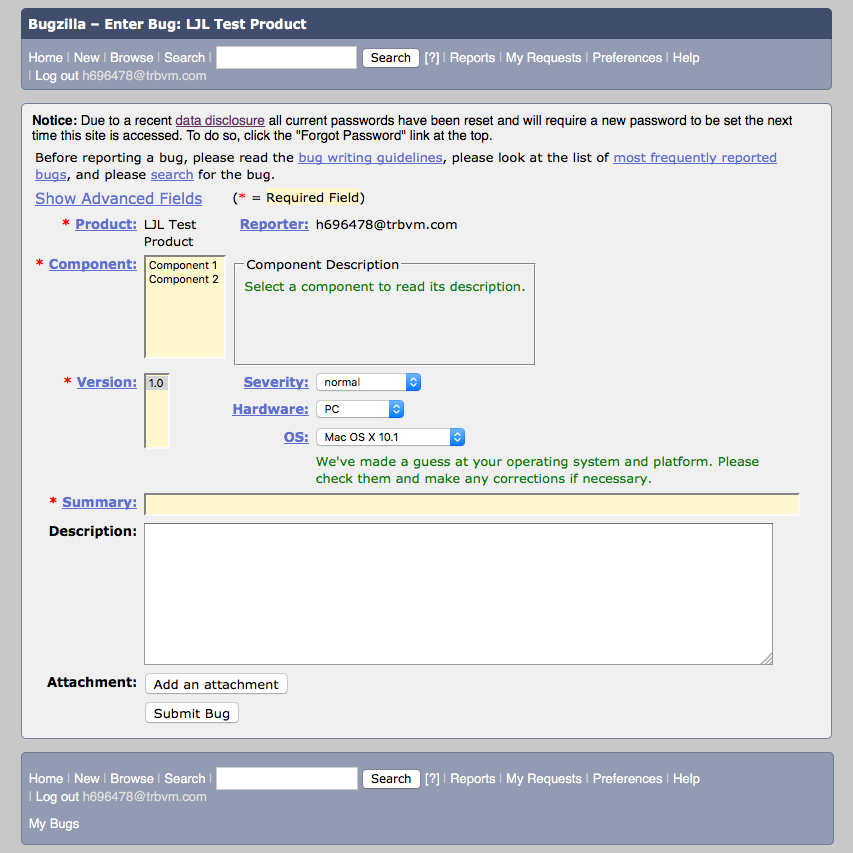
\includegraphics[width=.7\linewidth]{related/bugzilla}
  \caption{An old Bugzilla submission form}
  \label{fig:bugzilla-interface}
%\end{wrapfigure}
\end{figure}

In 1998, the Mozilla Foundation released the first version of \bzilla, which would soon become the reference issue tracking system. During the years different alternative tools emerged, providing their own set of customizations and personalizations. We briefly present four platforms, selected by importance and overall adoption, showing their salient features: \bzilla, \jira, the \gth issue tracker and \fbz.

\mypar{Bugzilla} \bzilla \seeurl{https://www.bugzilla.org} is one of the oldest and most popular issue tracking systems, that inspired many existing issue trackers. Developed by the Mozilla Foundation, it is used by several open source projects, as well as industrial customers. \bzilla allows a great level of detail in specifying an issue, thus producing, however, a complex interface, as shown in \figref{fig:bugzilla-interface}.

\mypar{JIRA} \jira by Atlassian\seeurl{https://www.atlassian.com/software/jira} is one of the most famous commercial issue trackers, used by Twitter, Linkedin, and Ebay. It provides a polished interface and strong integration with the tools developed by the company. It uses a model similar to \bzilla.

%\begin{wrapfigure}[9]{r}{0.45\textwidth}
%\centering
%  \vspace{-12pt}
%  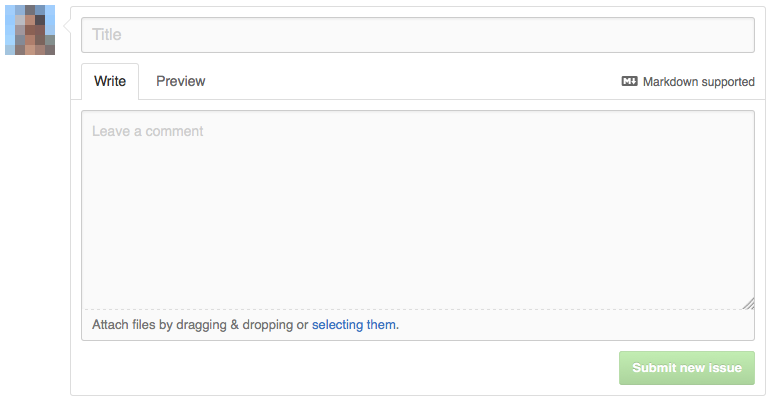
\includegraphics[width=.95\linewidth]{images/github}
%  \caption{GitHub Bug Submission Form}
%  \label{fig:github-interface}
%\end{wrapfigure}

\mypar{GitHub} \gth is a popular \texttt{Git} repository hosting service, used to develop several popular open source projects, that offers a simple issue tracker. \gth adopts a simplified model of a bug report, but offers a strong integration with the versioned source code, by linking issues with specific commits.

%\paragraph{\bf FogBugz.} \fbz\seeurl{https://www.fogcreek.com/fogbugz} is an issue tracker developed by FogCreek. I uses a bug model similar to \bzilla, slightly polished and user-friendly, due to its clean user interface and advanced filtering capabilities. It poses a strong accent on customization, by letting users define custom filters and views.

\paragraph{}
%\bf Other platforms}
Together with these platform, the open source and commercial scenes provide other popular solutions, like \textsc{FogBugz}, \textsc{Redmine} or \textsc{Trac}\footnote{\url{https://www.fogcreek.com/fogbugz}, \url{https://redmine.org/}, \url{http://trac.edgewall.org/}}. It is however interesting to observe that, while these systems propose different degrees of integration with the tools in their ecosystem (\eg the versioning system), the fundamental approach they adopt follows the same paradigm made popular by \bzilla: a textual description with additional customizable metadata. Further improvements to issue trackers, and the research around them, are built on top of this paradigm. In the following section, we present the efforts to improve issue trackers and their use in support the bug fixing activity.


\section{Bug Reports}

Dealing with bug reports is a non-trivial task, that poses a number of communication problems among users and developers. Such a large, noisy, and sometimes redundant corpus of information, impacts the debugging time and the maintenance costs. To minimize this impact, researchers focused on improving several aspects of this process. In the following, we present the results of research in selected areas, that represent the core aspects to compose a smart issue tracking system.


\mypar{Quality of a Bug Report}

The reliability and completeness of bug reports is crucial to quickly solve a defect. Bissyande \etal showed that most reporters that contribute to a project are not developers~\cite{Biss2013}, posing a problem on the quality of the data. To understand how developers perceive the quality of a bug report, researchers conducted a survey, asking which elements help understanding a problem. They found that stack traces are the most useful item and often contribute to a faster resolution of a defect, suggesting that they should be collected and included in issue trackers~\cite{Zimm2010a,Bett2007,Schr2010}. Even when reliable, though, the amount of information in an issue tracker can hide the relevant information: To alleviate the information overload, Sun devised a technique to detect bug reports without useful information~\cite{Sun2011}. Besides incorrect information, bug repositories often contain duplicate entries for the same defect. However, developers do not consider this harmful, but instead find the additional information useful to better understand the problem~\cite{Bett2008a}.
%\paragraph{\bf Automating the Information Management.}

Managing a large bug repository is often a burden that adds a new layer of complexity on top of the bug fixing problem. To alleviate this burden, researchers proposed to use automated approaches~\cite{Weim2006}. For example, Anvik \etal observed that large open source projects are often overwhelmed by the rate of new bug reports and proposed a machine learning based approach to to aid bug \emph{triaging} decisions~\cite{Anvi2006a}, the process of selecting the a the right person to take care of an issue.

%Guo \etal conducted a study to predict what impacts the resolution time of \textit{MS Windows} bug reports~\cite{Guo2010}, finding that a high number of reassignment of a report usually increases the issue lifetime, and that the reputation of the submitter also impacts the fixing time. Given the expensive nature of the bug fixing activity, a number of approaches exist to estimate the cost of a bug fix in person-hours~\cite{Weis2007}, predict bug fixing time~\cite{Gige2010}, locate features from bug reports \cite{Dit2013a}, and perform traceability linking \cite{Biss2013a}.


\mypar{Relevance of Bug Reports}

An important element to reduce the time needed to close a defect comes not only from filtering the relevant reports inside issue trackers, but also from the collection of valuable information.
To support the reliability of the collected information, both researchers and developers implemented tools to collect runtime exceptions to analyze runtime errors. For example, Glerum \etal used an automated approach to leverage the errors collected through WER, the \emph{Windows Error Reporting} tool~\cite{Glerum2009}. In their approach they grouped these reports into buckets, that they used to prioritize debugging and build a knowledge base where system administrators could check common problems of the system. Han Shi~\etal applied the same principle to performance debugging~\cite{Han2012}: They proposed an approach called \textsc{StackMine}, designed to detect and report performance bugs and address defects that cause delays in the user experience. Mozilla adopts a similar approach to collect stack traces and for debugging purposes~\cite{McLa2004}.

The information of stack traces contained in bug reports represents a valuable support in debugging: as such, many researchers devised different methods to aid bug fixing and management of reports using stack traces. These studies provided evidence that stack traces are useful tools and a precious source of information~\cite{Davie2013,Wang2013,Brod2005,Weis2007}, as they provide precise information, usually more reliable and useful than the descriptions produced by the submitter of a bug report~\cite{Ko2006}. Moreno \etal applied Text Retrieval techniques to compute similarity between bug reports using the stack traces in the report description, focusing on reducing the overhead to analyze large amounts of data~\cite{Moreno2014}.

%We believe that collecting stack traces and leveraging runtime data is a valuable support for developers in a programming environment, and should be part of the standard set of features of an issue tracking system.



\mypar{Understanding Bug Reports}

Having obtained meaningful and reliable data, it is important to build tools to make use of this information. Accessing the information in a bug report is a difficult step in the debugging process: The large amount of information and the reliability of the data reported by the users, consume a significative amount of developers' time. To alleviate this burden, researchers devised a number of approaches based on the visualization of the data inside issue trackers. D'Ambros \etal analyzed the \bzilla bug repository and synthesized a state transitions diagram of a report~\cite{DAmb2007b}. They built visualizations to support the analysis of a bug database at different levels of granularity, that depicts bug reports as independent entities. Their approach allows users to browse the history of an issue tracker and inspect parts of the system with custom filters. Knab \etal proposed visualizations to ease the understanding of the data in an issue tracker and find hidden patterns~\cite{Knab2009,Knab2010}. Hora \etal proposed a visual exploration of the bug repository, considering bugs as first class entities, and linking them to other software artifacts~\cite{Hora2012}. All these approaches focus on retrospective analyses. We believe that while conceptually interesting, there is little practical utility in daily development, since after all the goal of an issue tracking system is not to look at defects, but to actually fix them. This implies that even the most elaborated techniques are of limited actionability, since the bug fixing process takes place in a different space, namely the integrated development environment (IDE). We believe that the use for a visualization is not to simply display the data, but to establish a first-class link to the development environment. 


\mypar{Bug Prediction}

Solving defects does not represent the end of life of the information inside issue trackers: Yin \etal show the danger of hidden complexity behind a bug report, finding that 4.8\% to 24.4\% of sampled fixes for post-release bugs introduced new defects~\cite{Yin2011a}. They also noted that ``Developers and reviewers for incorrect fixes usually do not have enough knowledge about the involved code'', and that ``27\% of the incorrect fixes are made by developers who have never touched the source code files associated with the fix''. Once a bug report gets closed, the data inside issue trackers can still contain valuable information, and has been exploited to predict the evolution of the code. D'Ambros \etal presented several approaches devised by researchers to predict future defects~\cite{DAmb2012a}. For example,  Zimmermann \etal proposed an approach based on network analysis on dependency graphs among components, to allow managers to identify central program units that are more likely to face defects~\cite{Zimm2008a}. Kim \etal suggested that defects tend to show in places previously affected by other defects, proposing a caching method to prioritize the elements in the code to inspect~\cite{Kim2007a}. It is the source code that contains the defects, but these defects are introduced through changes: As such, Hassan \etal proposed metrics for bug prediction that consider the changes in the code, rather than the code itself~\cite{Hass2009a}.


Despite the efforts in improving the accuracy of the bug predicton approaches, Bhattacharya and Neamtiu showed the low correlation of current prediction techniques and underlined the need to find additional features to increase the confidence of the time estimates~\cite{Bhat2011}.


\mypar{Bug Reports and Social Interactions}

One of the core aspects of an issue tracker is that it collects social interactions in a community: Users can give feedback to the developers and obtain information on the system. Breu \etal analyzed a sample of 600 bug reports, finding that interacting with developers helps solving an issue faster~\cite{Breu2010}. Zhou and Mockus showed that users involved in the development activity, like bug reporting and participating in the community, are more likely to become stable, long time contributors~\cite{Zhou2015}. Therefore, improving issue trackers to foster the relations between developers and users could result in faster resolution of defects.


\section{Research Areas}

Issue tracking is a central and time consuming part of the development activity: Therefore, the proposed improvements and research areas that revolve around issue trackers are vast.
%For example, researchers focused on detection of duplicate bug reports, identifying the roles and expertise of the users,
We selected the aspects presented in this section because we think that they are relevant in shaping an issue tracker and the processes that compose the workflow of a developer. Our main focus is to improve the representation of the information and its reliability, to allow a quick comprehension of the contents of a bug report, reducing the amount of incorrect information. A quick access to the information would speed up the fixing process, while lowering the effort needed to approach a bug report, thus allowing new users to contribute more easily to the development of a project.

This selection represents a minimal viable core of features, to build the blueprints for a new issue tracking system, that can be later be extended to include further approaches. In the next chapter we outline such a system, including in its design the practices adopted in modern issue tracking, to adapt to the current challenges in software development.


